%============================================================================%
% DOCUMENT DEFINITION
%============================================================================%
\documentclass[12pt,a4paper,english]{article}

%-----------------------------------------------------------------------------
% Page layout
%-----------------------------------------------------------------------------
% page outer frames (debug-only)
% \usepackage{showframe}

% define page styles using geometry
\usepackage[a4paper]{geometry}

% Margins
\geometry{top=2cm, bottom=2cm, left=1cm, right=1cm}

%-----------------------------------------------------------------------------
% Packages
%-----------------------------------------------------------------------------
% Math
\usepackage{amsmath}

% Extended implementation of the arrays and tabules
\usepackage{array}

% Languages
\usepackage[main=english, spanish]{babel}
\usepackage[spanish]{datetime2}
\usepackage{indentfirst}

% Enhances the quality of tables.
\usepackage{booktabs}

% To use the slash to cancel out stuff
\usepackage{cancel}

% Customise the captions in figures and table
\usepackage{caption}

% Enumeration
\usepackage{enumitem}

% fancy headers and footers
\usepackage{fancyhdr}

% Improves the interface for defining floating objects such as figures and tables.
\usepackage{float}
\restylefloat{table}
\usepackage{diagbox}

% The enhanced graphics package.
\usepackage{graphicx}
\graphicspath{{./}{./images}{./figures}} % Default graphics path
\DeclareGraphicsExtensions{.pdf, .png, .jpg} % Extensions to read in order

% Hyper links
\usepackage[hidelinks]{hyperref}

% Fonts
% \usepackage[semibold]{raleway}
% \usepackage{lmodern}
% \usepackage[defaultsans]{droidsans}
% \usepackage{cmbright}
% \usepackage[light,math]{iwona}

% Select font encodings.
\PassOptionsToPackage{T1}{fontenc} % T2A for cyrillics
\usepackage{fontenc}

% Select  input encodings.
\PassOptionsToPackage{utf8}{inputenc}
\usepackage{inputenc}

% Code listings
\usepackage{accsupp}
\newcommand{\noncopy}[1]{\BeginAccSupp{method=escape,ActualText={}}#1\EndAccSupp{}}

\usepackage[most]{tcolorbox}
\usepackage{listings}
\usepackage{minted}
\usemintedstyle{perldoc}
\renewcommand{\theFancyVerbLine}{\sffamily{\scriptsize {\arabic{FancyVerbLine}}}}

% Columns
\usepackage{multicol}

% Set the 5-point spacing between paragraphs and 20-point indent for the first line.
\usepackage[skip=5pt plus1pt, indent=20pt]{parskip}

% High-quality function plots
\usepackage{pgfplots}
\pgfplotsset{compat=1.18}
\usepgfplotslibrary{dateplot}

% TikZ
\usepackage{tikz}
\usetikzlibrary{shapes.geometric, arrows}

% Easily annotate math equations using TikZ
\usepackage{annotate-equations}

% Named colors
\usepackage[dvipsnames,table]{xcolor}

% Conditional space
\usepackage{xspace}

\let\OldTexttrademark\texttrademark
\renewcommand{\texttrademark}{\OldTexttrademark\xspace}%

% Fancy quotations
\usepackage[style=british]{csquotes}
\def\signed #1{{\leavevmode\unskip\nobreak\hfil\penalty50\hskip1em
    \hbox{}\nobreak\hfill #1%
    \parfillskip=0pt \finalhyphendemerits=0 \endgraf}}

\newsavebox\mybox
\newenvironment{aquote}[1]
    {\savebox\mybox{#1}\begin{quote}\openautoquote\hspace*{-.7ex}}
    {\unskip\closeautoquote\vspace*{1mm}\signed{\usebox\mybox}\end{quote}}

%-----------------------------------------------------------------------------
% Re-usable information
%-----------------------------------------------------------------------------
\newcommand{\myName}{Dmitry Ivanov\xspace}%
\newcommand{\myEmail}{divanov@correo.ugr.es\xspace}%
\newcommand{\myDate}{\datespanish\today\xspace}%
\newcommand{\myTitle}{2D geometric data types\xspace}%
\newcommand{\mySubject}{EDGSG 23/24\xspace}%
\newcommand{\myKeyWords}{Geometric Algorithms\xspace}%

\title{\mySubject\\\myTitle}
\author{\myName (\myEmail)}
\date{\today}

%-----------------------------------------------------------------------------
% Header
%-----------------------------------------------------------------------------
\pagestyle{fancy}
\setlength{\headheight}{28pt}
\fancyhead[LO,L]{\mySubject\\\myTitle}
\fancyhead[CO,C]{}
\fancyhead[RO,R]{\myName(\myEmail)\\\today}
\fancyfoot[LO,L]{}
\fancyfoot[CO,C]{\thepage}
\fancyfoot[RO,R]{}
\renewcommand{\headrulewidth}{0.4pt}
\renewcommand{\footrulewidth}{0.4pt}

%-----------------------------------------------------------------------------
% PDF information
%-----------------------------------------------------------------------------
\hypersetup{
  pdfauthor = {\myName (\myEmail)},
  pdftitle = {\myTitle},
  pdfsubject = {\mySubject},
  pdfkeywords = {\myKeyWords},
  pdfcreator = {Visual Studio Code with TeX Live 2023},
  pdfproducer = {pdflatex}
}

\newcommand{\BlueHref}[3][blue]{\href{#2}{\color{#1}{#3}}}%

\usepackage{titlesec}
\titleformat{\section}{\normalsize\bfseries}{\thesection.}{0.5em}{}
\titlespacing{\section}{0em}{*4}{*1.5}

\titleformat{\subsection}{\normalsize\itshape}{\alph{subsection}.}{0.5em}{}
\titlespacing{\subsection}{2em}{*4}{*1.5}

%============================================================================%
% DOCUMENT CONTENT
%============================================================================%
\begin{document}

\section{Introduction}
I've made a couple of improvements to the project to provide a unified way to compile the project on Windows and Linux.
Moreover, I've added a square perimeter and circumference random distribution to random utilities to draw squared and round point clouds.

I've included precompiled binaries for Windows and Linux.

\section{Compilation on Windows}

\begin{itemize}
    \item Install Visual Studio from \url{https://visualstudio.microsoft.com/downloads/}
    \item Install VCPKG from \url{https://vcpkg.io/en/getting-started.html}
    \item Add VCPKG folder to PATH:
    \item Option 1: Command Line tools

    \begin{minted}[fontsize=\small,mathescape,linenos,frame=single,xleftmargin=20pt,xrightmargin=20pt,numbersep=0.2em]{Batch}
    REM Assuming that VCPKG cloned and bootstrapped in c:\src\vcpkg
    REM setx for the global environment, set for the local
    setx PATH c:\src\vcpkg;%PATH%
    set  PATH c:\src\vcpkg;%PATH%
    \end{minted}

    \item Option 2: PowerShell
    \begin{minted}[fontsize=\small,mathescape,linenos,frame=single,xleftmargin=20pt,xrightmargin=20pt,numbersep=0.2em]{Powershell}
    # Assuming that VCPKG cloned and bootstrapped in c:\src\vcpkg
    [Environment]::SetEnvironmentVariable("PATH", "c:\src\vcpkg;${PATH}", "Machine")
        Set-Item -Path Env:PATH -Value "c:\src\vcpkg;${PATH}"
    \end{minted}

    \item Option 3: Manually in \textbf{System Properties \text{-->} Environment Variables}
    \item Navigate to the folder with the project
    \item Run \textit{build.bat}
    \item Open \textit{build\\EDGSG.sln} in Visual Studio to work with the source code
\end{itemize}

\section{Compilation on Linux}

\begin{itemize}
    \item Install VCPKG from \url{https://vcpkg.io/en/getting-started.html}
    \item Add VCPKG folder to System PATH
    \item Option 1: Temporary local environment
    \begin{minted}[fontsize=\small,mathescape,linenos,frame=single,xleftmargin=20pt,xrightmargin=20pt,numbersep=0.2em]{Bash}
        # Assuming that VCPKG cloned and bootstrapped in ~/vcpkg
        export PATH="~/vcpkg;${PATH}"
    \end{minted}

    \item Option 2: Local environment and Bash profile
    \begin{minted}[fontsize=\small,mathescape,linenos,frame=single,xleftmargin=20pt,xrightmargin=20pt,numbersep=0.2em]{Bash}
        # Assuming that VCPKG cloned and bootstrapped in c:\src\vcpkg
        export PATH="~/vcpkg;${PATH}"
        echo 'export PATH="~/vcpkg;${PATH}"' >> ~/.bashrc
    \end{minted}

    \item Navigate to the folder with the project
    \item Run build.sh
\end{itemize}
\textbf{Important Note:} the VCPKG requests installation of additional packages

\section{Point Clouds}

\begin{figure}[H]
    \centering
    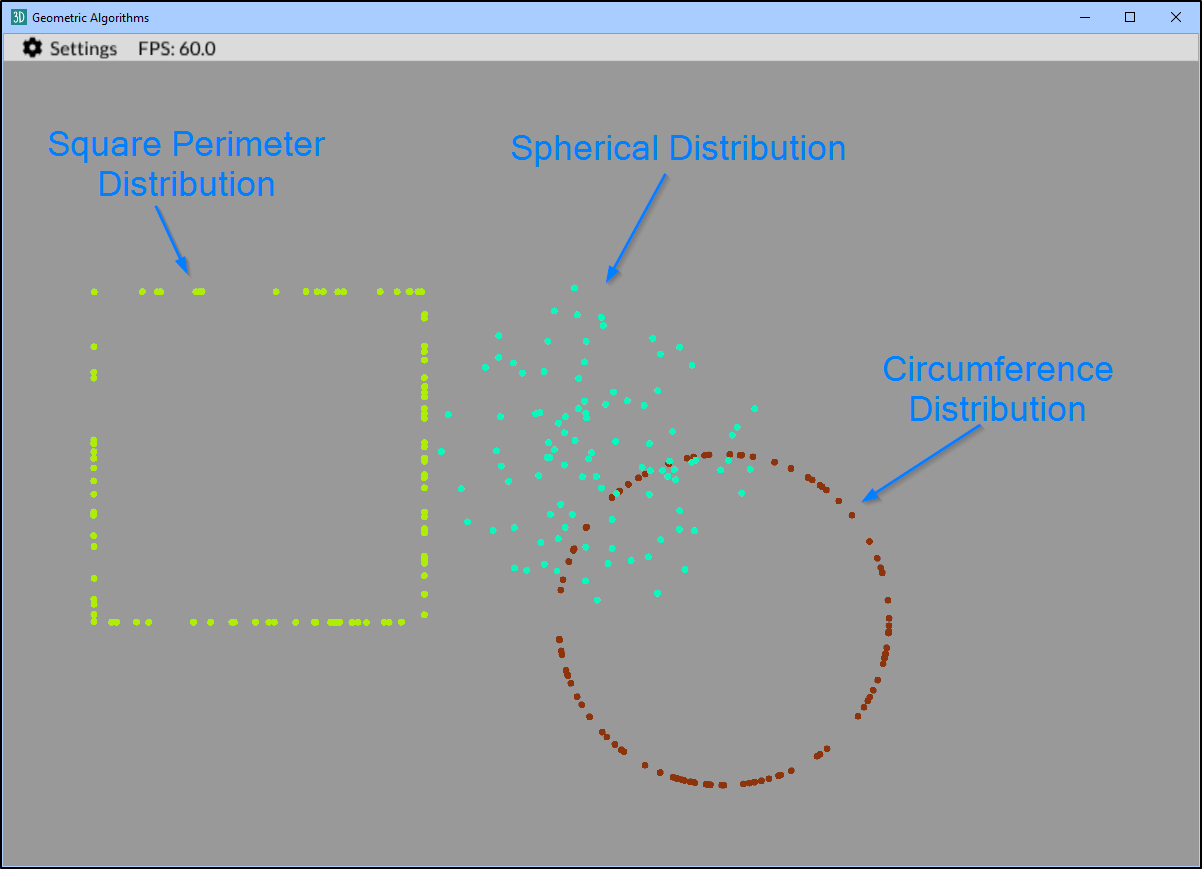
\includegraphics[width=0.8\textwidth]{point_cloud}
    \caption[]{Point Clouds.}
    \label{fig:point_cloud}
\end{figure}

I've included multiple ways to generate point clouds: using Hemispherical random distribution, Spherical random distribution, circle random distribution, and square random distribution. The first point cloud is generated in a Spherical manner. Following point clouds are smaller and generated squarely for uneven point cloud IDs and circle manner for even IDs.

Point clouds could be saved to a file and loaded to a file using the following pattern:

\begin{minted}[fontsize=\small,mathescape,linenos,frame=single,xleftmargin=20pt,xrightmargin=20pt,numbersep=0.2em,highlightlines={1,4}]{C++}
    auto* pointCloud = new PointCloud("PointCloud" + std::to_string(pcIdx) + ".txt");
    ...
    ...
    pointCloud->save("PointCloud" + std::to_string(pcIdx) + ".txt");
\end{minted}

\section{Segment, Ray, Line}

\begin{figure}[H]
    \centering
    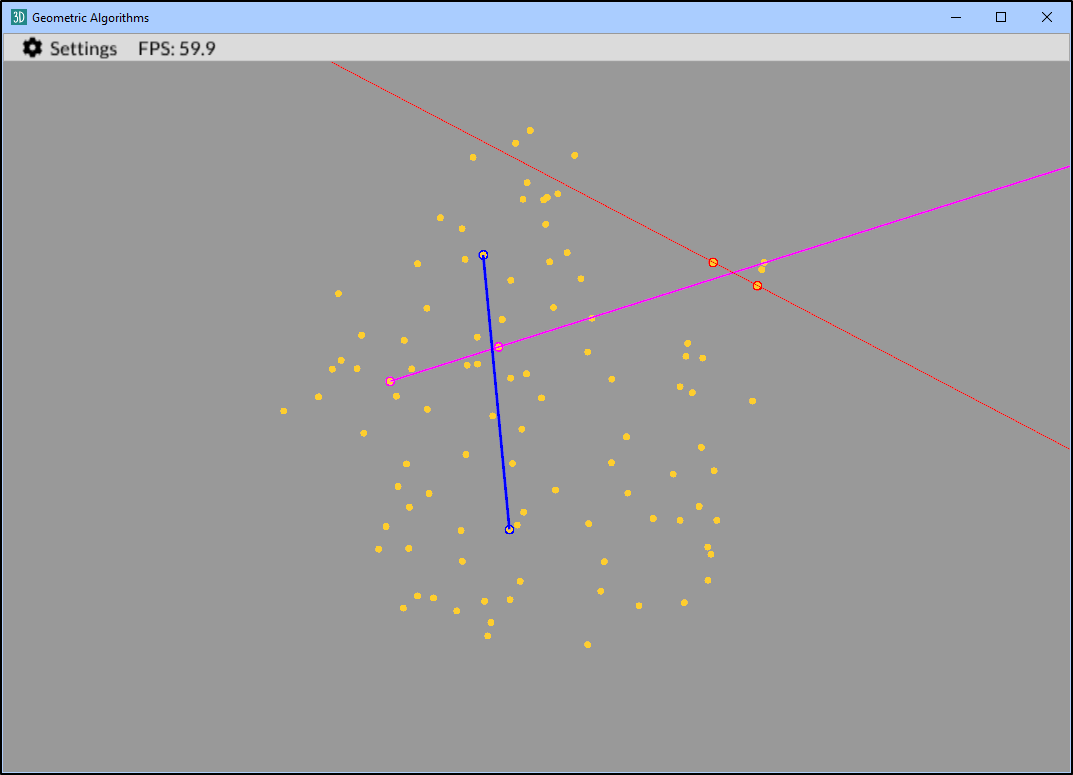
\includegraphics[width=0.8\textwidth]{segment_ray_line}
    \caption[]{Blue Segment, red Line, and magenta Ray.}
    \label{fig:segment_ray_line}
\end{figure}

To generate Segment, Ray, and Line, I've taken 6 random points from the central point cloud. The point selection is totally random, so one point, potentially, can belong to all three objects. To distinguish them, I draw them in different sizes. Additionally, I draw the origin and destination points in bigger sizes to emphasize them.

\section{Convex Polygon}

\begin{figure}[H]
    \centering
    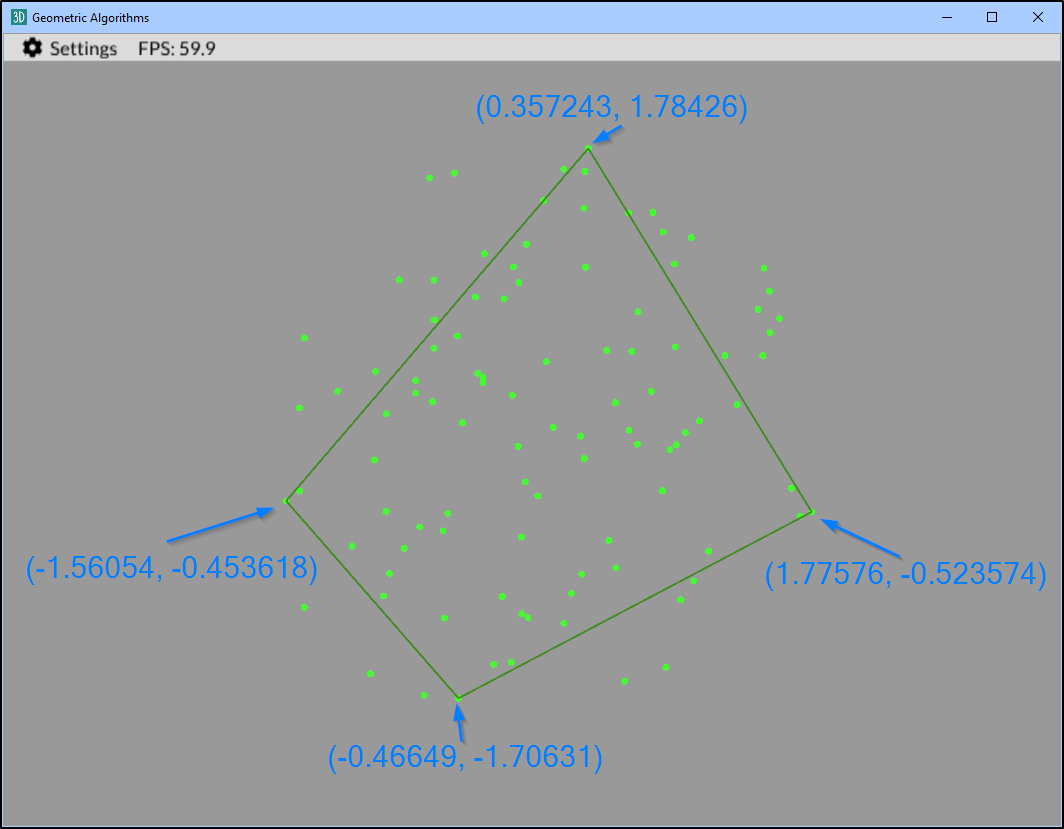
\includegraphics[width=0.8\textwidth]{convex_polygon}
    \caption[]{Convex Polygon from 4 points of point cloud.}
    \label{fig:convex_polygon}
\end{figure}

Four points for convex were selected from the point cloud using maximum and minimum x and y values.

\section{Bezier Curve}

\begin{figure}[H]
    \centering
    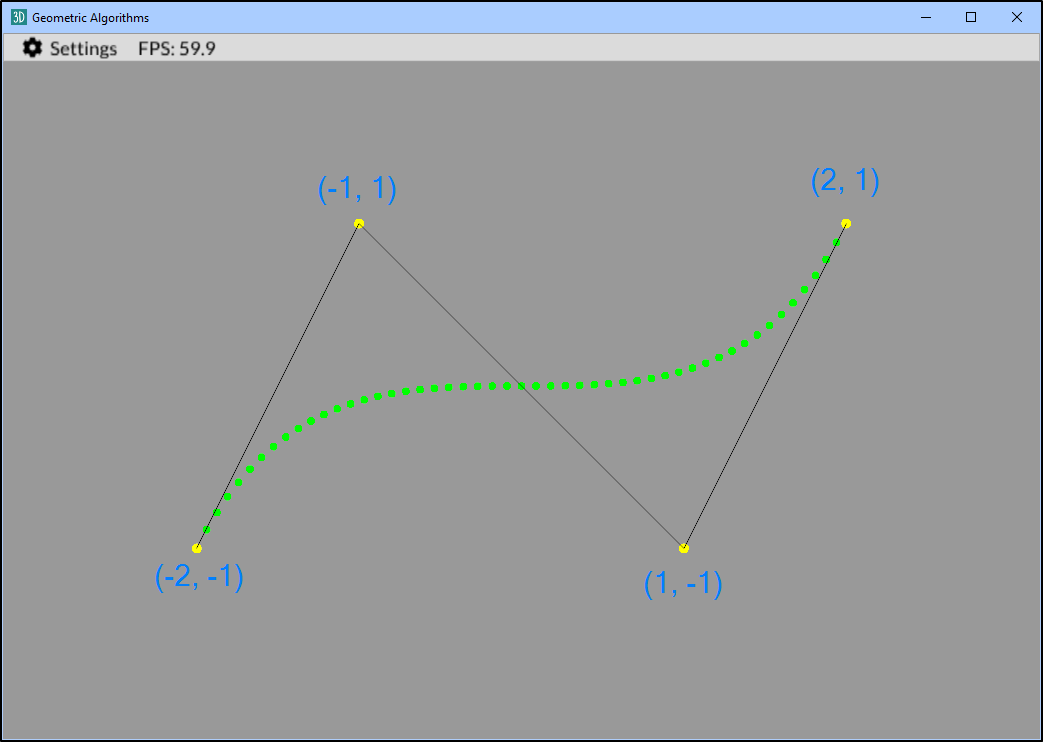
\includegraphics[width=0.8\textwidth]{bezier_curve}
    \caption[]{Bezier Curve.}
    \label{fig:bezier_curve}
\end{figure}

I've provided commented-out predefined points for the Bézier curve. In the picture, I've carefully selected them to show the beauty of the Bézier curve. The point cloud could be used as a source of control points, but there are too many to make a good curve. Additionally, I draw control points and control segments.

\section{Everything on one picture}

\begin{figure}[H]
    \centering
    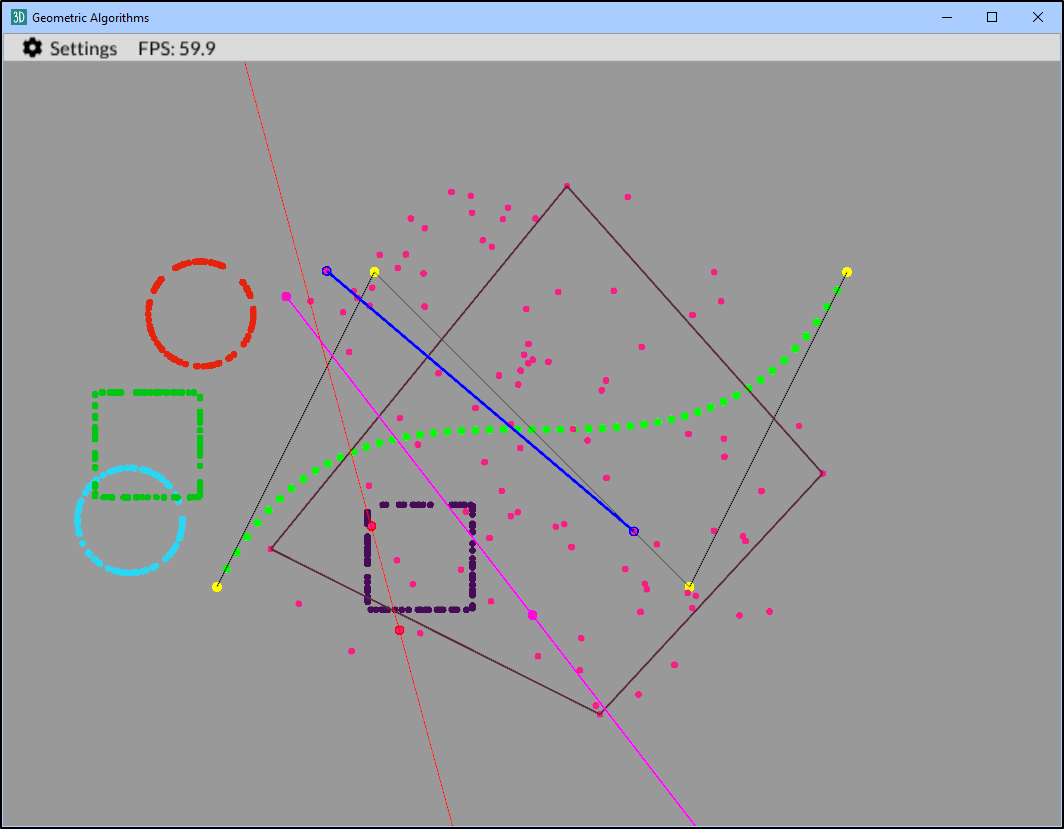
\includegraphics[width=0.8\textwidth]{all_in_one}
    \caption[]{All in one.}
    \label{fig:all_in_one}
\end{figure}

\end{document}
